\documentclass[UTF8,11pt,a4paper]{ctexart}

% --- 基础宏包 ---
\usepackage{graphicx}
\usepackage{caption}
\usepackage{fancyhdr}
\usepackage{amsmath, amssymb, amsfonts}
\usepackage[a4paper, left=3.17cm, right=3.17cm, top=2.54cm, bottom=2.54cm]{geometry}
\usepackage{xcolor}
\usepackage{booktabs, array, longtable, multirow}
\usepackage[numbers,sort&compress,super]{natbib}
\usepackage{float}
\usepackage{enumitem}
\usepackage{tabularx}
\usepackage{filecontents}
\usepackage{hyperref}
\setcitestyle{open={[},close={]},super}

% --- 1. 标题与段落设置 ---
\ctexset{
  section = {
    format = \zihao{3}\heiti\bfseries\centering,
    name = {第,章},
    number = \arabic{section},
    aftername = \hspace{1em},
    beforeskip = 24pt,
    afterskip = 18pt
  },
  subsection = {
    format = \zihao{-3}\heiti\raggedright,
    aftername = \hspace{1em},
    beforeskip = 24pt,
    afterskip = 6pt
  },
  subsubsection = {
    format = \zihao{4}\heiti\raggedright,
    aftername = \hspace{1em},
    beforeskip = 12pt,
    afterskip = 6pt
  },
  bibname = {参考文献}
}

\renewcommand{\baselinestretch}{1.33}

% --- 参考文献标题与条目格式 ---
\renewcommand{\bibsection}{
    \section*{\centering\zihao{3}\heiti\bfseries 参考文献}
    \addcontentsline{toc}{section}{参考文献}
    \vspace{6pt}
}
\providecommand{\bibfont}{}
\renewcommand{\bibfont}{\fontsize{10.5pt}{16pt}\selectfont}
\setlength{\bibsep}{0pt}

% --- 2. 页眉页脚设置 ---
\pagestyle{fancy}
\fancyhf{}
\newcommand{\xiaowu}{\fontsize{9pt}{11pt}\selectfont}

\fancyhead[L]{
    \begin{minipage}[b]{0.6\textwidth}
        \includegraphics[height=0.63cm]{tjlogo.png}
    \end{minipage}
}

\fancyhead[R]{
    \xiaowu
    {2353125 郑凯博~~\\
     ~《大数据与数据工程》课程大作业报告}
}

\fancyfoot[C]{\thepage}
\renewcommand{\headrulewidth}{0.5pt}

% --- 3. 消除红框设置 ---
\hypersetup{
    colorlinks=true,
    linkcolor=black,
    citecolor=black,
    urlcolor=blue!70!black,
    hidelinks
}

% --- 中文摘要环境设置 ---
\newenvironment{cnabstract}{
    \newpage
    \pagenumbering{Roman}
    \section*{\centering\zihao{3}\heiti\bfseries 摘要}
    \addcontentsline{toc}{section}{摘要}
    \zihao{-5}\songti\linespread{1.33}\selectfont
}{
    \par
}

\newcommand{\cnkeywords}[1]{
    \vspace{1em}
    \noindent {\zihao{-5}\heiti\bfseries 关键词：} #1
}

% --- 英文摘要环境保留，当前课程报告不使用 ---
\newenvironment{enabstract}{
    \newpage
    \section*{\centering\zihao{3}\bfseries Abstract}
    \addcontentsline{toc}{section}{Abstract}
    \zihao{-4}\linespread{1.33}\selectfont
}{
    \par
}

\newcommand{\enkeywords}[1]{
    \vspace{1em}
    \noindent {\zihao{-4}\bfseries Key Words:} #1
}

% 定制附录页面的标题样式
\newcommand{\setupappendix}{
    \ctexset{
        section = {
            format = \zihao{3}\heiti\bfseries\centering,
            name = {附录},
            number = \Alph{section},
            beforeskip = 24pt,
            afterskip = 18pt
        }
    }
    \renewcommand{\thefigure}{\Alph{section}.\arabic{figure}}
    \renewcommand{\thetable}{\Alph{section}.\arabic{table}}
    \renewcommand{\theequation}{\Alph{section}.\arabic{equation}}
}

\begin{filecontents*}{\jobname.bib}
@misc{tianchi2026ccks,
  author       = {{阿里云天池}},
  title        = {{CCKS2026-任务六：大模型生成文本检测及溯源}},
  howpublished = {\url{https://tianchi.aliyun.com/competition/entrance/532474}},
  year         = {2026}
}
@article{he2021debertav3,
  author  = {He, Pengcheng and Gao, Jianfeng and Chen, Weizhu},
  title   = {{DeBERTaV3}: Improving {DeBERTa} using {ELECTRA}-Style Pre-Training with Gradient-Disentangled Embedding Sharing},
  journal = {arXiv preprint arXiv:2111.09543},
  year    = {2021}
}
@inproceedings{hu2022lora,
  author    = {Hu, Edward J. and Shen, Yelong and Wallis, Phillip and Allen-Zhu, Zeyuan and Li, Yuanzhi and Wang, Shean and Wang, Lu and Chen, Weizhu},
  title     = {{LoRA}: Low-Rank Adaptation of Large Language Models},
  booktitle = {International Conference on Learning Representations},
  year      = {2022}
}
@inproceedings{wolf2020transformers,
  author    = {Wolf, Thomas and Debut, Lysandre and Sanh, Victor and others},
  title     = {Transformers: State-of-the-Art Natural Language Processing},
  booktitle = {Proceedings of the 2020 Conference on Empirical Methods in Natural Language Processing: System Demonstrations},
  pages     = {38--45},
  year      = {2020}
}
@inproceedings{paszke2019pytorch,
  author    = {Paszke, Adam and Gross, Sam and Massa, Francisco and others},
  title     = {{PyTorch}: An Imperative Style, High-Performance Deep Learning Library},
  booktitle = {Advances in Neural Information Processing Systems},
  volume    = {32},
  year      = {2019}
}
@article{pedregosa2011scikit,
  author  = {Pedregosa, Fabian and Varoquaux, Ga{\"e}l and Gramfort, Alexandre and others},
  title   = {Scikit-learn: Machine Learning in Python},
  journal = {Journal of Machine Learning Research},
  volume  = {12},
  pages   = {2825--2830},
  year    = {2011}
}
\end{filecontents*}

%==============================================================================
\begin{document}

\begin{titlepage}
    \centering

    \vspace{1.0cm}

    \includegraphics[height=3.0cm]{tjlogo.png}

    \vspace{2.5cm}

    {
        \zihao{-4}\heiti \textbf{基于 DeBERTa-LoRA 的大模型生成文本检测与溯源系统} \par
    }

    \vspace{1.5cm}

    {\zihao{5} 大数据与数据工程 \par}
    \vspace{0.5cm}
    {\zihao{5} 课程大作业报告 \par}

    \vspace{3cm}

    {\zihao{5}
    \begin{tabular}{cc}
        \textbf{学生专业：} & 人工智能 \\[0.8em]
        \textbf{学生学号：} & 2353125 \\[0.8em]
        \textbf{学生姓名：} & 郑凯博\\[0.8em]
    \end{tabular}
    \par}

    \vfill

    \begin{center}
    {\zihao{5} \today} \\ \vspace{0.5cm}
    \end{center}

    \thispagestyle{empty}
\end{titlepage}

\newpage
\pagenumbering{Roman}

\addtocontents{toc}{\protect\setcounter{tocdepth}{-10}}

\begin{cnabstract}

随着大语言模型在教育、科研、媒体和社交平台中快速普及，文本真实性判断与生成来源追踪成为数据治理中的重要问题。本文以 CCKS2026 天池“任务六：大模型生成文本检测及溯源”为案例，围绕训练数据获取、JSONL 数据存储、数据统计分析、可视化展示、模型训练、推理提交与结果管理，完成了一个完整的数据工程实践项目。项目使用训练集 98,800 条文本和测试集 A 12,350 条文本，任务包括三分类检测，即纯人类撰写、纯机器生成与人机协作文本，并在机器生成文本上进一步识别 8 个大模型家族。方法上，本文先实现 TF-IDF + SGD 作为可解释基线，再基于 DeBERTa-v3-large 构建 LoRA 参数高效微调模型，并设计融合 CLS、均值池化、最大池化和注意力池化的风格感知分类头，以同时捕捉语义内容与生成风格线索。实验结果显示，最终模型在本地验证集上取得检测 Macro-F1 0.9922、溯源 Macro-F1 0.8797，按官方加权公式估计综合分数为 0.9697。该案例体现了课程中数据获取、数据处理、统计分析、可视化和模型实现的综合应用。

\cnkeywords{大模型生成文本检测；文本溯源；数据工程；DeBERTa；LoRA}

\end{cnabstract}

\addtocontents{toc}{\protect\setcounter{tocdepth}{3}}

\newpage
\tableofcontents

\newpage
\pagenumbering{arabic}
\setcounter{page}{1}
\zihao{5}\songti
\setlength{\parindent}{2em}
\setlength{\parskip}{0.45em}
\renewcommand{\arraystretch}{1.2}

\section{案例背景介绍}

大语言模型能够在极短时间内生成结构完整、语义连贯且风格自然的文本。这一能力在提升内容生产效率的同时，也带来了新的数据治理问题：一段文本究竟出自人类撰写、模型生成，还是人机协作？若文本由模型生成，又应归因于哪一个模型家族？这些问题不仅是典型的文本分类问题，更直接关系到教育诚信、新闻真实性、平台内容审核以及人工智能生成内容（AIGC）的版权归属。

本文选取 CCKS2026 天池“任务六：大模型生成文本检测及溯源”作为课程大作业案例\cite{tianchi2026ccks}。该任务要求系统对输入文本进行两级判断：首先完成三分类检测，区分纯人类文本、纯机器文本与人机协作文本（依次记为标签 0、1、2）；当文本被判定为纯机器生成时，进一步识别其所属的模型家族（记为 0 至 7）。这一设定将文本真实性判别与生成来源归因有机串联，官方评价采用检测任务与溯源任务的加权 Macro-F1：
\[
  \mathrm{Score}=0.8 \times F1_{\mathrm{detect}}+0.2 \times F1_{\mathrm{source}}.
\]
其中检测任务为主要得分来源，溯源任务虽权重较低，但仍对最终成绩具有显著影响。

从课程视角看，本项目并不局限于训练单一的深度学习模型，而是完整覆盖了数据工程的多个环节，包括原始数据整理、数据格式统一、统计分析、可视化展示、模型训练、分布式运行、实验日志管理、指标汇总以及提交文件生成。图 \ref{fig:motivation} 概括了本项目的现实动机：多源文本在进入可信文本生态之前，需要依次经过检测与溯源两个关键环节。

\begin{figure}[H]
  \centering
  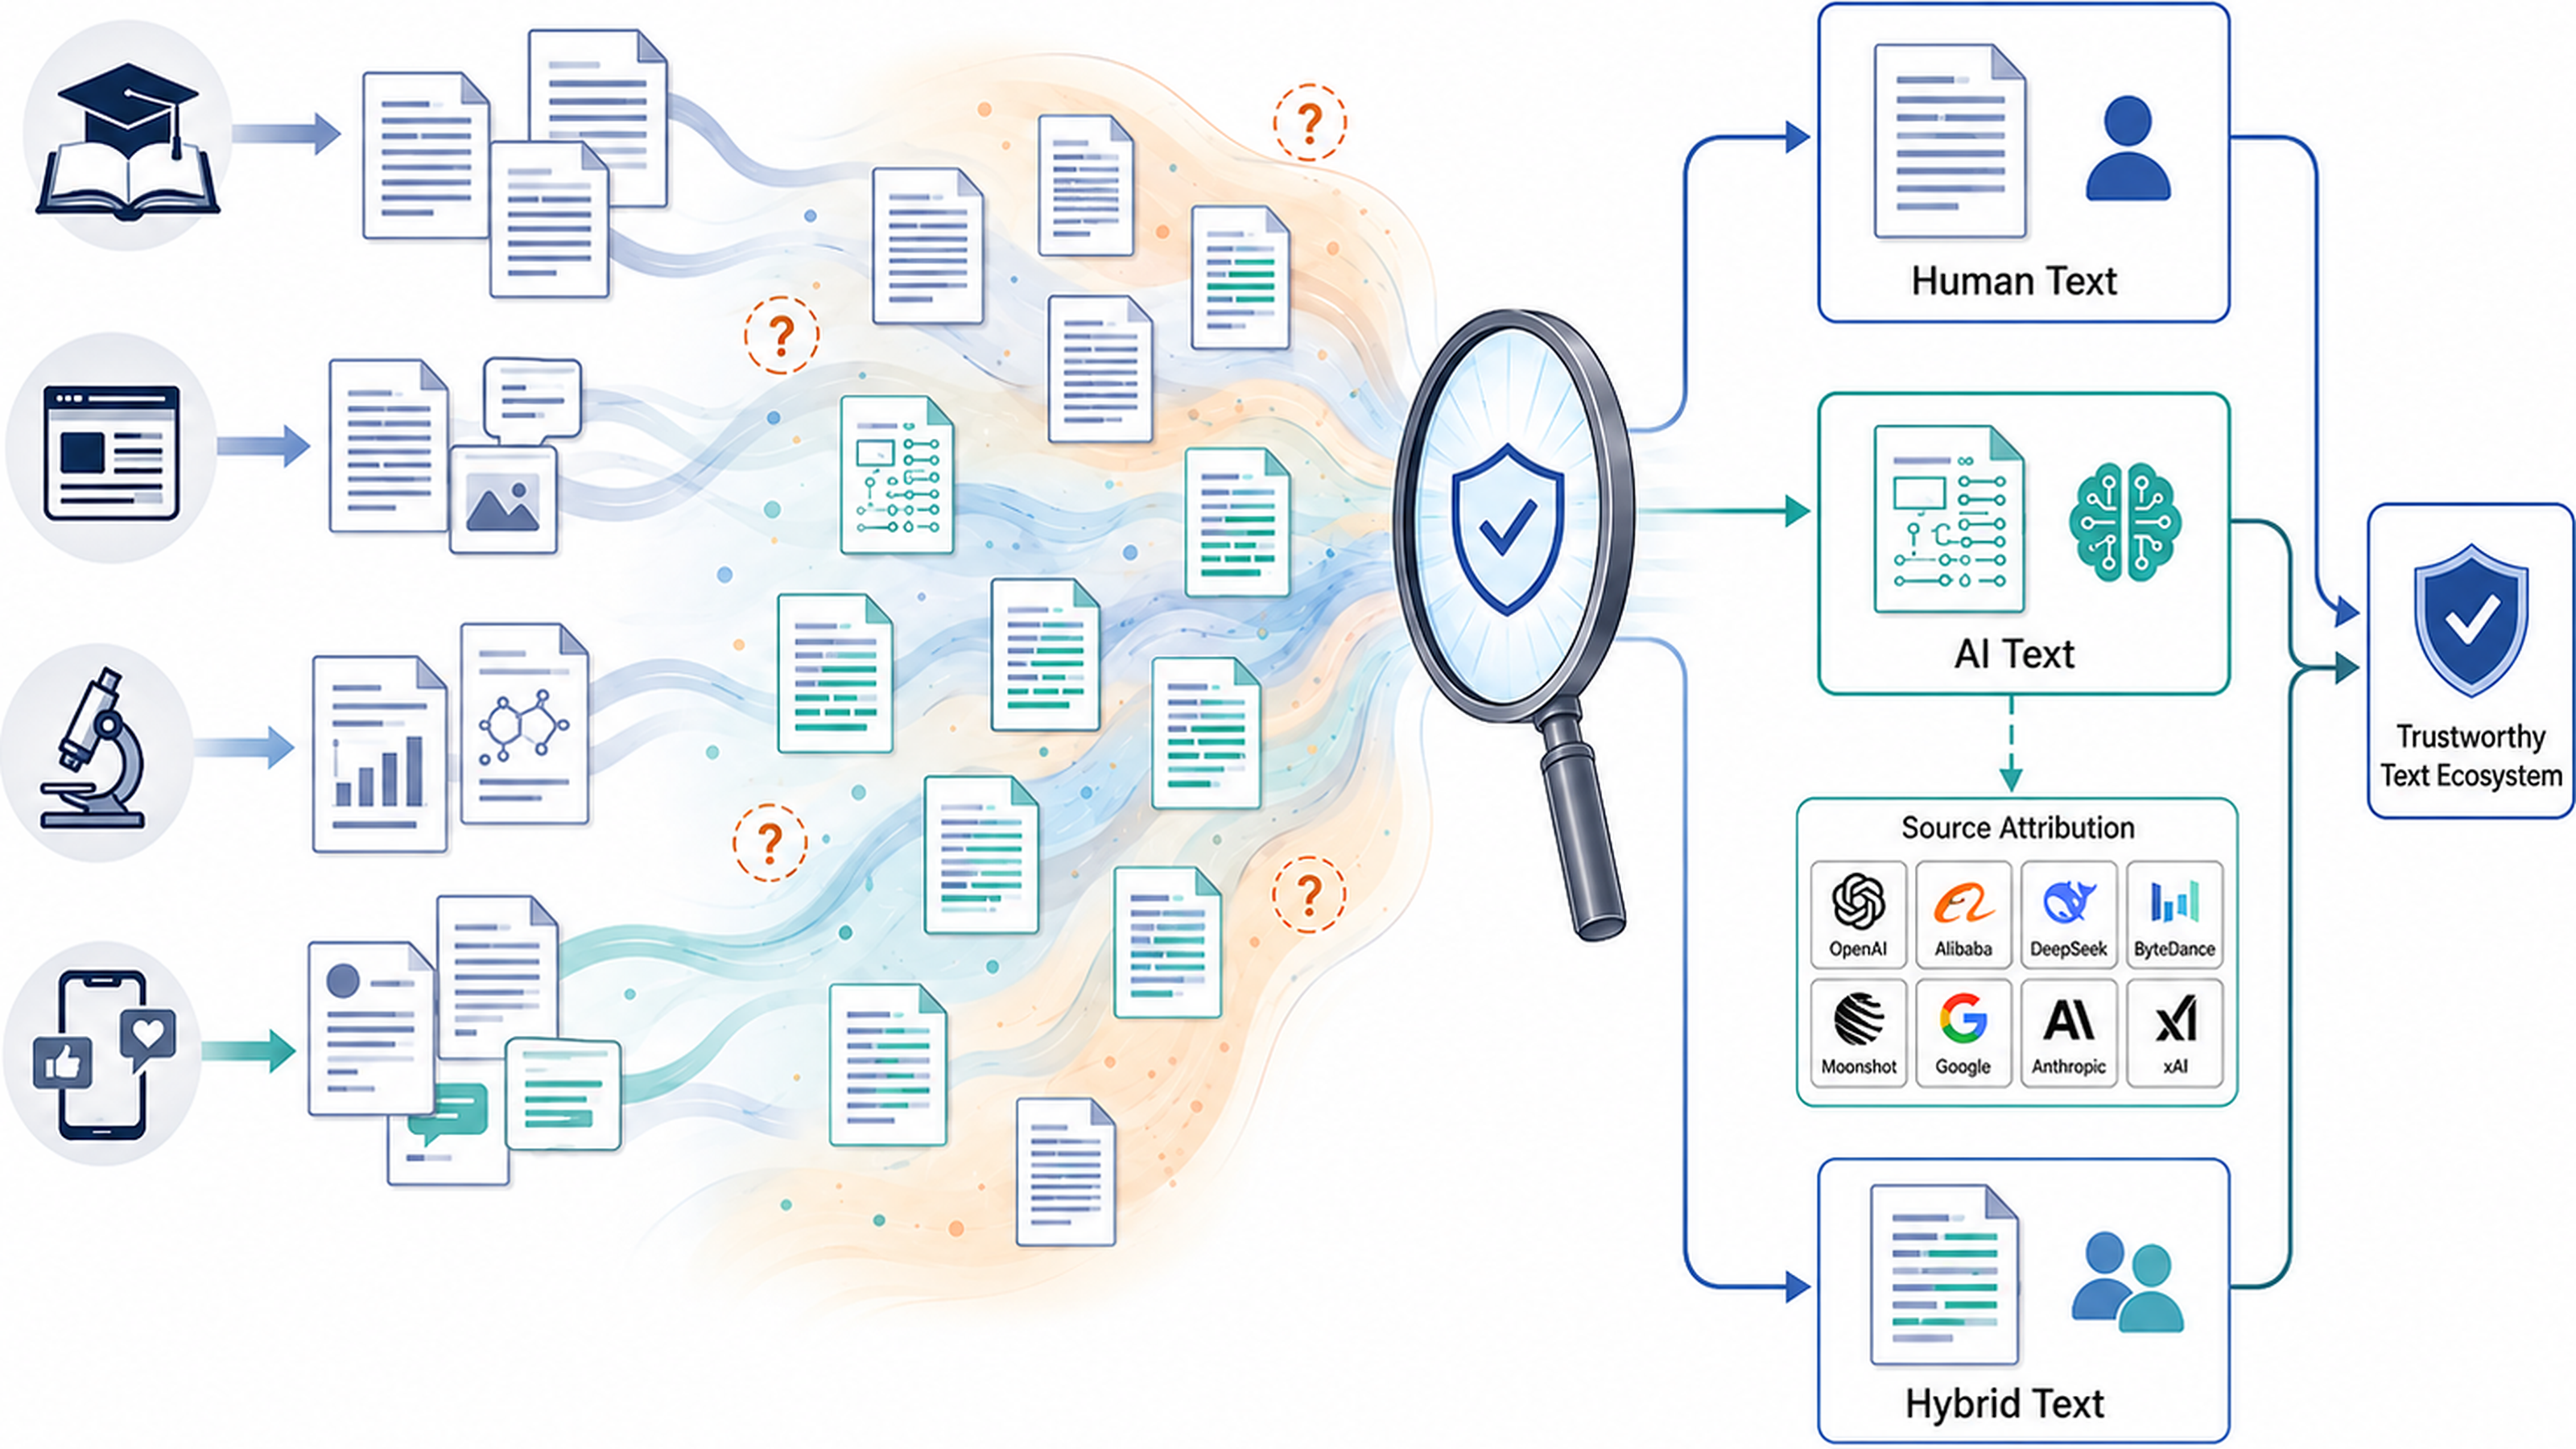
\includegraphics[width=0.98\textwidth]{../Illustration/1.png}
  \caption{项目动机：面向可信文本生态的大模型生成文本检测与模型家族溯源。}
  \label{fig:motivation}
\end{figure}

\section{案例相关数据集描述}

本项目使用的原始数据由训练集与测试集 A 两部分组成，均以 JSONL 格式存储，每行对应一个独立的 JSON 对象，便于流式读取与大规模文本处理。训练集中每条样本包含编号、正文文本与检测标签等字段；纯机器文本额外标注其生成模型及所属家族，人机协作文本则记录相应的协作构造方式。这种字段组织方式使检测与溯源能够被自然地拆解为两个相互关联的监督学习子任务。测试集 A 仅提供待预测文本及其编号，最终需据此生成符合官方格式的提交文件。两份数据的基本规模如表 \ref{tab:data} 所示。

\begin{table}[H]
  \centering
  \begin{tabular}{lrrrr}
    \toprule
    数据集 & 文件名 & 样本数 & 文件大小 & 平均词数 \\
    \midrule
    训练集 & \path{train.jsonl} & 98,800 & 159.0 MB & 258.6 \\
    测试集 A & \path{test_a_release.jsonl} & 12,350 & 19.4 MB & 258.6 \\
    \bottomrule
  \end{tabular}
  \caption{数据集规模统计}
  \label{tab:data}
\end{table}

训练集中三类检测标签的分布较为均衡，纯人类文本、纯机器文本与人机协作文本分别为 32,000、32,000 与 34,800 条。纯机器文本进一步均匀划分为 8 个模型家族，每个家族 4,000 条，分别对应 OpenAI、Alibaba、DeepSeek、ByteDance、Moonshot、Google、Anthropic 与 xAI。人机协作文本则按协作方式细分，涵盖机器改写人类文本、人类与机器文本混合、以及机器续写人类文本前缀等多种构造形式。

为充分了解数据特性，本文对训练集与测试集进行了系统的统计分析，结果如图 \ref{fig:data} 所示，涵盖数据规模、标签分布、模型家族分布、文本长度分布以及人机协作方式分布。统计结果为后续建模提供了重要依据：检测任务的类别相对均衡，适合以 Macro-F1 作为评价指标；溯源任务中各家族样本数量同样均衡，但不同模型家族之间的文本风格差异更为细微，需要比传统词频特征更具判别力的语义与风格表示。

\begin{figure}[H]
  \centering
  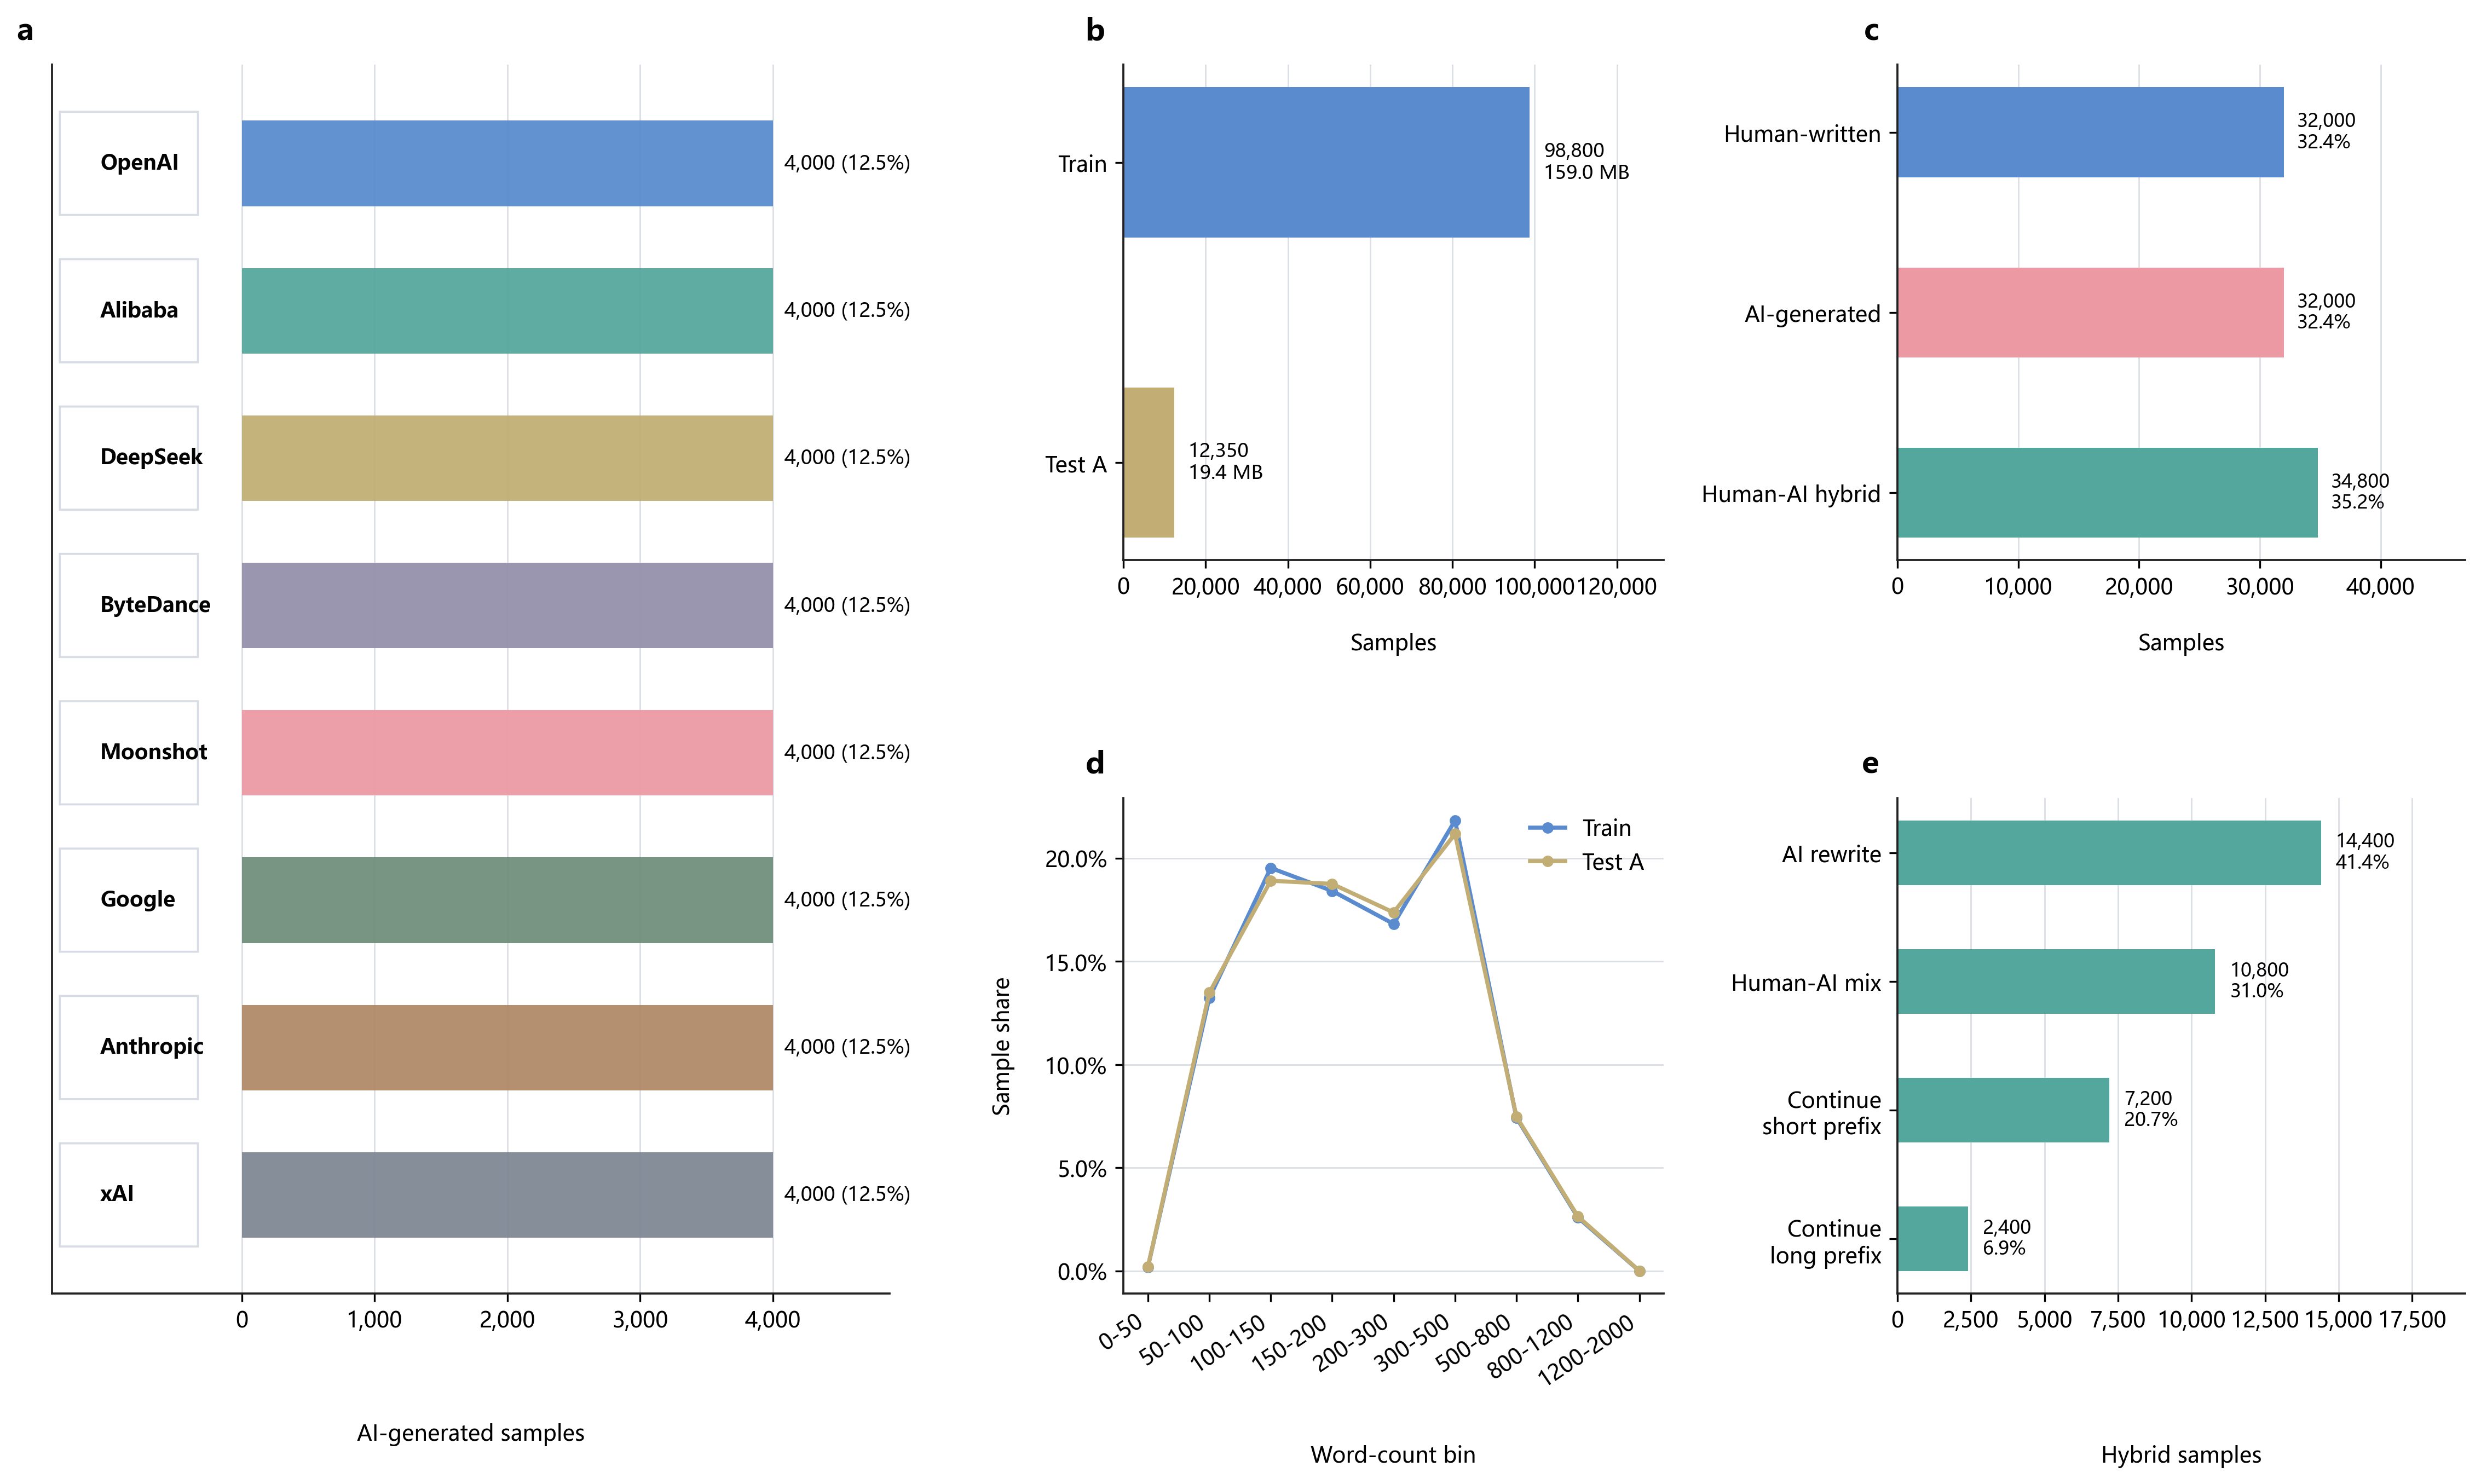
\includegraphics[width=0.98\textwidth]{../Illustration/2.png}
  \caption{数据集分析：训练与测试规模、标签分布、模型家族分布、文本长度分布及协作方式分布。}
  \label{fig:data}
\end{figure}

\section{案例涉及的模型与方法实现}

\subsection{基线模型}

本文首先实现 TF-IDF 结合 SGD 线性分类器的方案作为基线模型。该方法将文本转化为词项权重向量，并分别针对检测任务与溯源任务训练线性分类器。其训练速度快、可解释性强，适合用于验证数据读取、标签映射、指标计算与提交格式的正确性，并为后续深度模型提供性能参照。基线模型在本地验证集上取得检测 Macro-F1 0.8945、溯源 Macro-F1 0.7079，表明简单的词频特征已能够捕捉部分生成文本的统计差异，但在细粒度的模型家族溯源上仍显不足。

\subsection{DeBERTa-LoRA 主模型}

主模型以 \path{microsoft/deberta-v3-large} 作为预训练文本编码器。DeBERTaV3 通过改进的预训练目标与解耦注意力机制，显著增强了上下文表示能力\cite{he2021debertav3}，适合处理细粒度文本分类任务。考虑到对大模型进行全参数微调存在参数规模大、显存开销高的问题，本文采用低秩适配（LoRA）方法，仅对注意力层中的查询、键、值投影矩阵注入低秩增量进行参数高效微调\cite{hu2022lora}。该策略在保留预训练模型原有能力的同时，大幅降低了可训练参数规模与训练成本。

在分类头设计上，本文不再仅依赖传统的 CLS 向量，而是引入风格感知池化头。设编码器输出的隐状态序列为 $H=[h_1,h_2,\ldots,h_n]$，分类头同时提取四种互补表示并加以拼接：
\[
z=\mathrm{Concat}\bigl(h_{\mathrm{CLS}},\ \mathrm{MeanPool}(H),\ \mathrm{MaxPool}(H),\ \mathrm{AttnPool}(H)\bigr).
\]
其中，CLS 向量保留整体语义，均值池化刻画全文的平均风格，最大池化捕捉局部的强响应片段，注意力池化则根据任务自适应地聚焦关键位置。拼接后的特征依次经过 LayerNorm、全连接层、GELU 激活与多样本 Dropout（Multi-sample Dropout），最终输出分类结果，从而在统一的分类头中融合全局语义与局部风格证据。模型整体结构如图 \ref{fig:model} 所示。

\begin{figure}[H]
  \centering
  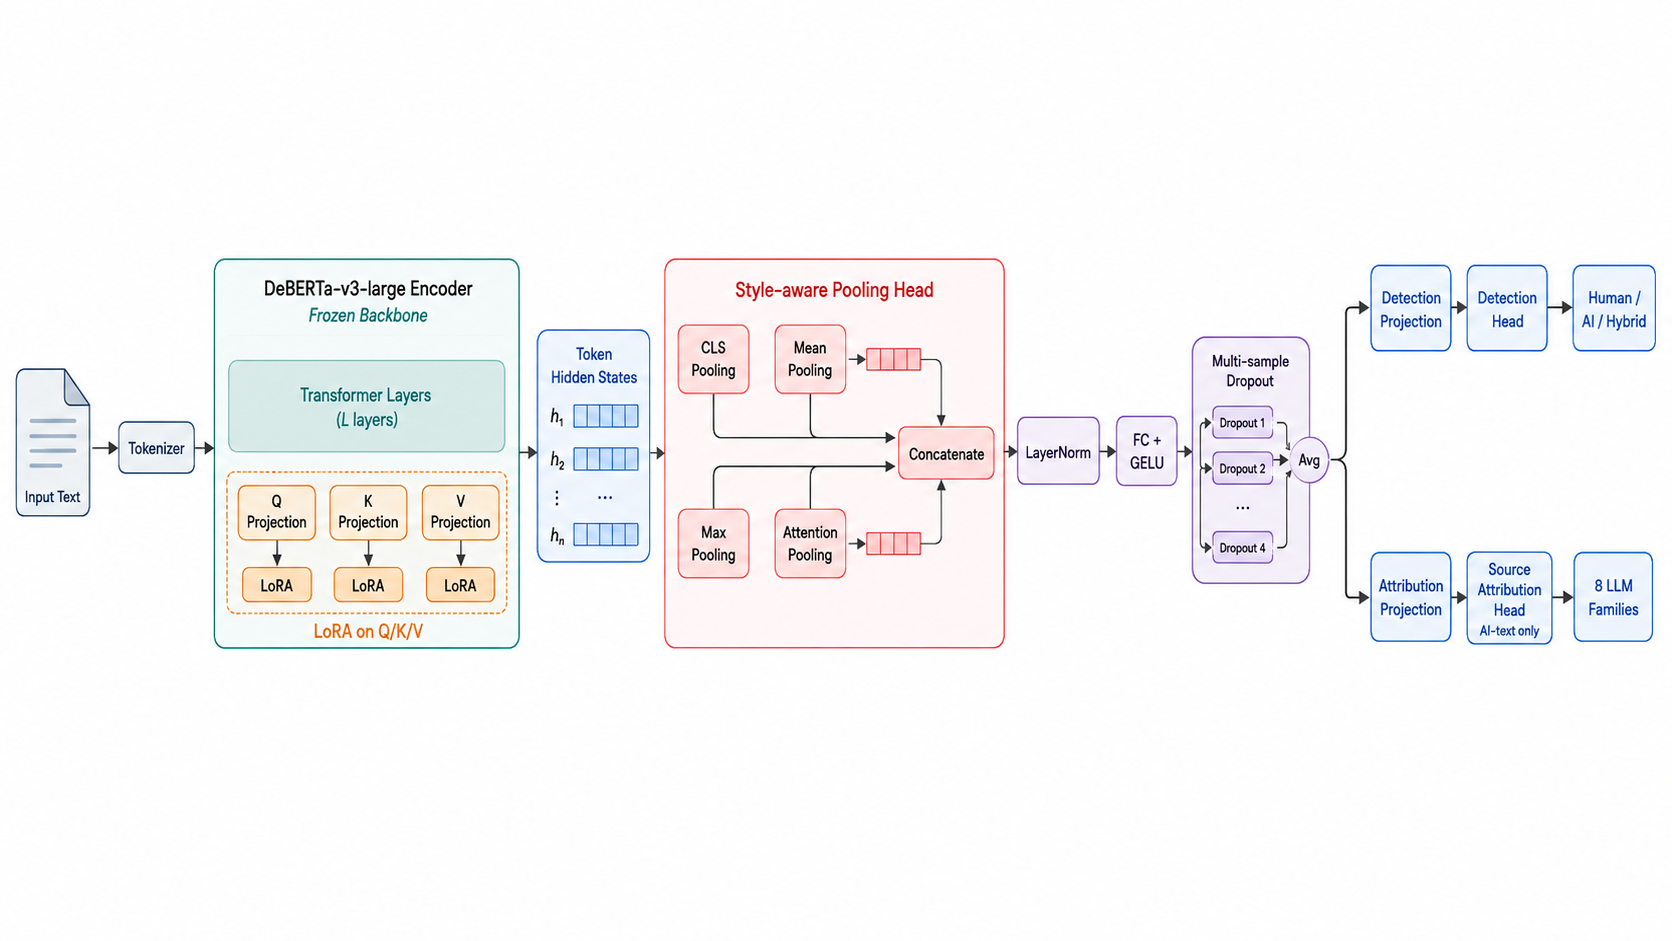
\includegraphics[width=0.98\textwidth]{../Illustration/3.png}
  \caption{模型结构：DeBERTa-v3-large 编码器、LoRA 微调与风格感知池化分类头。}
  \label{fig:model}
\end{figure}

\section{案例实现过程}

本项目按照深度学习竞赛的工程规范组织，将数据、训练、推理、模型资产与实验结果分目录管理，以保证训练、评估与归档各环节之间的路径关系清晰、流程可复现。整体实现可划分为数据分析、基线实验、主模型训练与推理提交四个阶段。

在数据分析阶段，本文对训练集与测试集进行统一的统计与质量检查，得到数据规模、标签分布、文本长度等画像信息，为建模与评价指标的选择提供依据。在基线实验阶段，本文构建 TF-IDF 与 SGD 分类器流水线，快速跑通从数据读取、标签映射到指标计算与提交文件生成的完整链路，从而确立性能基准。

主模型训练阶段针对检测与溯源两个子任务分别训练独立的 LoRA 适配器。检测适配器在全部训练样本上学习三分类任务；溯源适配器仅在纯机器文本子集上学习 8 类家族归因，从而与官方“仅对机器文本溯源”的设定保持一致。两个适配器共享同一冻结的 DeBERTa-v3-large 主干，仅在低秩增量与风格感知分类头上进行训练。为提升训练效率，正式实验采用单机多卡的分布式数据并行（DDP）方式，在 4 张 NVIDIA RTX 5090 显卡上完成，并通过运行日志与 Weights \& Biases 对训练过程进行监控。所用的深度学习与机器学习工具库包括 PyTorch\cite{paszke2019pytorch}、Transformers\cite{wolf2020transformers} 与 scikit-learn\cite{pedregosa2011scikit}。正式实验的主要超参数设置见表 \ref{tab:hyper}。

\begin{table}[H]
  \centering
  \begin{tabular}{ll}
    \toprule
    配置项 & 取值 \\
    \midrule
    训练轮数 & 20 \\
    最大序列长度 & 384 \\
    最大字符截断 & 8000 \\
    单卡训练批大小 & 16 \\
    梯度累积步数 & 1 \\
    评估批大小 & 64 \\
    LoRA 秩 $r$ & 16 \\
    LoRA 缩放系数 $\alpha$ & 32 \\
    LoRA 学习率 & $8\times10^{-5}$ \\
    分类头学习率 & $8\times10^{-4}$ \\
    \bottomrule
  \end{tabular}
  \caption{正式实验的主要超参数设置}
  \label{tab:hyper}
\end{table}

在推理提交阶段，系统采用两级流程生成最终结果：首先由检测适配器对测试集文本预测检测标签；对于被判定为纯机器的文本，再由溯源适配器预测其模型家族，其余文本的家族字段则置为 $-1$。最终预测结果按官方要求写入提交文件 \path{submit.jsonl}。完整的运行命令见附录。

\section{实验结果与分析}

本地评价基于从训练集中划分出的验证集进行。其中，检测任务的验证集包含 9,880 条样本，溯源任务的验证集包含 3,200 条纯机器样本。各方法在本地验证集上的主要结果如表 \ref{tab:results} 所示。

\begin{table}[H]
  \centering
  \begin{tabular}{lccc}
    \toprule
    方法 & 检测 Macro-F1 & 溯源 Macro-F1 & 加权估计分数 \\
    \midrule
    TF-IDF + SGD & 0.8945 & 0.7079 & 0.8572 \\
    DeBERTa-LoRA 初始版 & 0.9178 & 0.3090 & 0.7961 \\
    DeBERTa-LoRA + 强分类头 & 0.9922 & 0.8797 & 0.9697 \\
    \bottomrule
  \end{tabular}
  \caption{各方法在本地验证集上的结果}
  \label{tab:results}
\end{table}

实验结果表明，TF-IDF + SGD 基线可作为有效的性能参照，但其语义表达能力有限。初始的 DeBERTa-LoRA 模型在检测任务上已优于基线，然而溯源任务表现明显偏弱，说明普通线性分类头难以充分利用模型家族之间细微的风格差异。引入风格感知池化头并进行更充分的训练后，检测 Macro-F1 提升至 0.9922，溯源 Macro-F1 提升至 0.8797，按官方加权公式估计的综合分数达到 0.9697，这进一步印证了多粒度文本表示对来源归因任务的重要价值。

在测试集 A 上，模型的预测分布总体合理，预测为人类文本、机器文本与人机协作文本的样本分别为 3,994、4,003 与 4,353 条，与官方测试集 A 的类别规模基本一致。图 \ref{fig:result} 给出了实验结果的总体概览，包括检测与溯源指标、溯源任务的训练曲线、测试集 A 的预测标签分布以及机器文本的家族预测分布。其中，溯源任务在第 19 轮训练时达到最佳 Macro-F1 0.8797，此后指标略有波动，表明模型在当前验证划分下已接近收敛。

\begin{figure}[H]
  \centering
  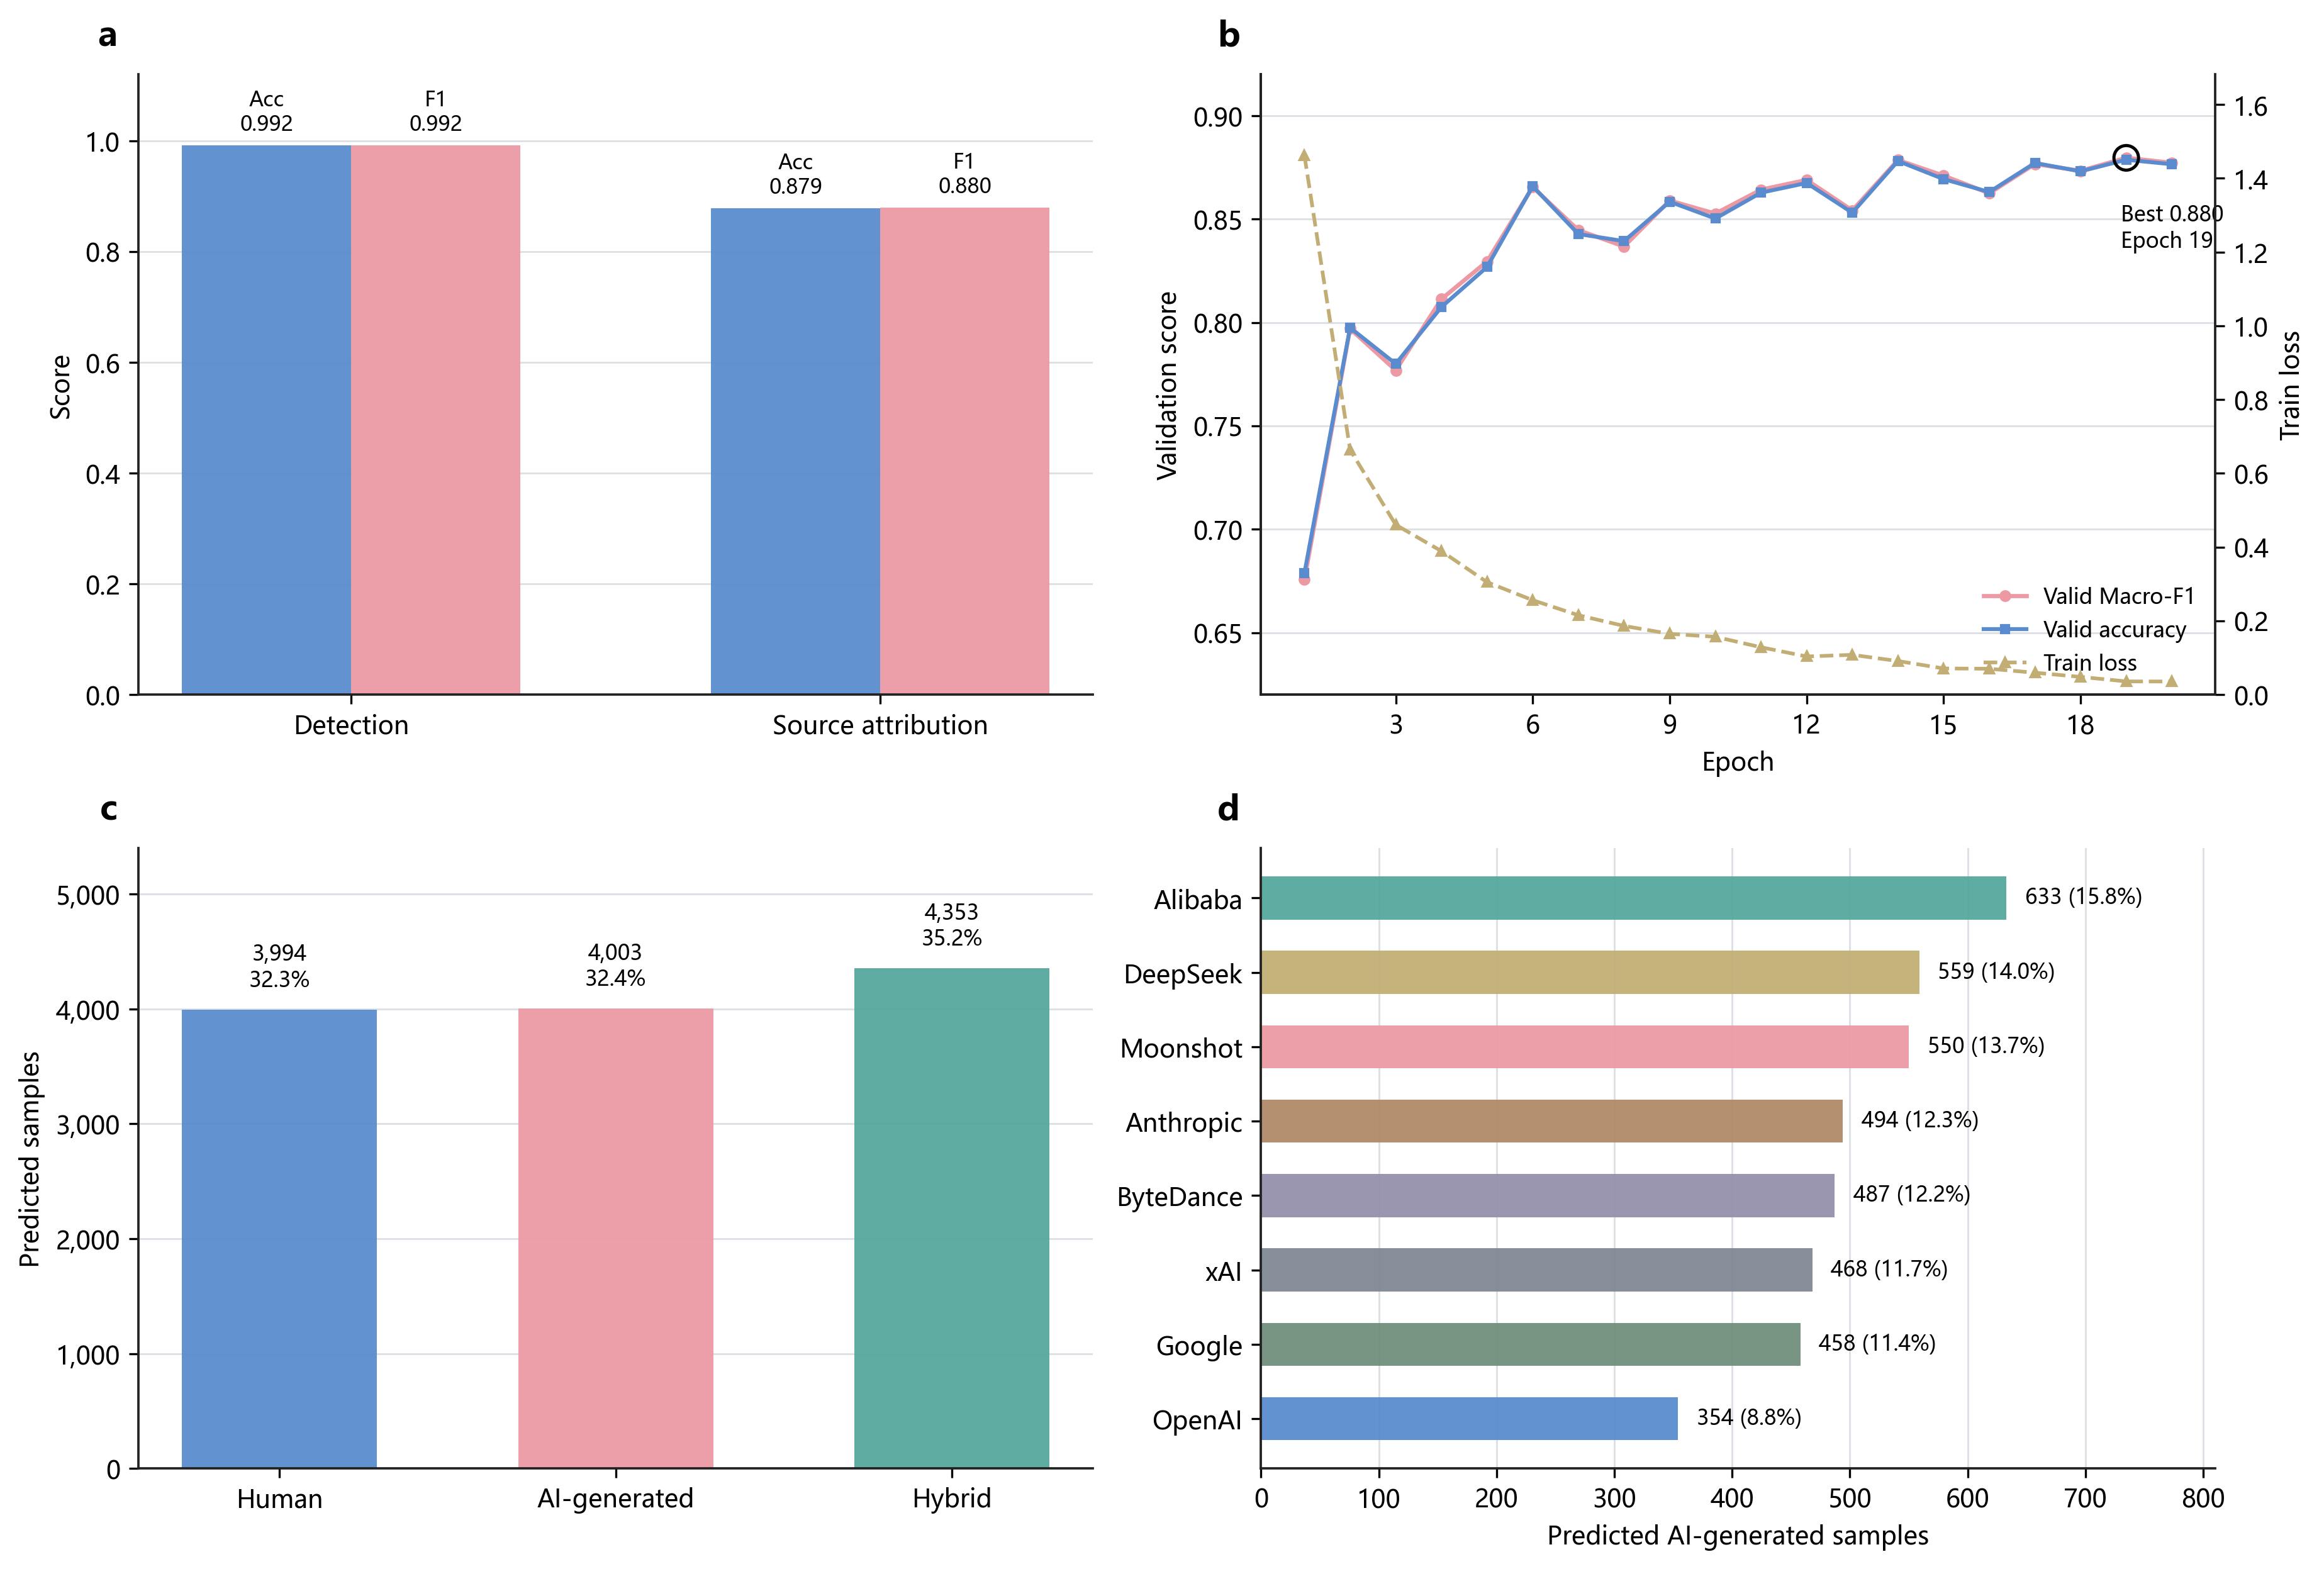
\includegraphics[width=0.98\textwidth]{../Illustration/4.png}
  \caption{实验结果汇总：验证指标、溯源训练曲线、测试集 A 预测标签与家族分布。}
  \label{fig:result}
\end{figure}

\section{改进思路}

针对本项目，后续工作可从以下五个方面进一步展开。其一，引入 K 折交叉验证与多随机种子训练，以降低单一数据划分带来的偶然性，并通过模型集成提升预测的稳定性。其二，开展更细致的错误分析，分别统计人机协作文本与纯机器文本之间的混淆、不同模型家族之间的误判，以及长文本截断对预测结果的影响。其三，尝试分段编码或长上下文模型，使模型能够同时利用文本开头、主体与结尾的风格信息。其四，在赛题规则允许的前提下，引入公开的 AIGC 检测数据进行领域自适应预训练，以增强模型对未知主题与未知生成器的泛化能力。其五，探索检测与溯源任务的联合训练，使检测任务学到的机器文本表示能够更直接地服务于家族溯源。

\section{结论}

本文围绕 CCKS2026 大模型生成文本检测及溯源任务，完成了一个面向课程大作业的数据工程与深度学习实践案例。项目从原始 JSONL 数据出发，构建了涵盖数据统计、可视化分析、基线实验、DeBERTa-LoRA 参数高效微调、多卡分布式训练、指标汇总与提交文件生成的完整流程。实验结果表明，参数高效微调结合风格感知分类头能够显著提升检测与溯源效果，在本地验证集上取得检测 Macro-F1 0.9922、溯源 Macro-F1 0.8797。该案例不仅体现了《大数据与数据工程》课程中数据获取、数据存储、数据处理、数据分析与结果可视化的综合应用，也说明了规范的项目结构与可复现的实验流程在竞赛类数据工程项目中的重要意义，为后续的实验复现与课程材料归档奠定了基础。

\newpage
\bibliographystyle{unsrtnat}
\bibliography{\jobname}

\newpage
\section{附录：提交材料与运行说明}

本项目的主要提交材料包括：源程序目录（\path{train/}、\path{eval/}、\path{tool/} 与 \path{visualization/}）、环境配置脚本、模型适配器目录 \path{ckpt/}、实验结果目录 \path{result/}、最终提交文件 \path{submit.jsonl}、报告插图目录 \path{Illustration/}，以及本报告源文件。课程提交前，可将报告 PDF、PPT、源程序、测试结果与数据说明一并压缩为“学号+姓名.zip”后上传。

完整实验流程可通过以下命令复现：

\begin{verbatim}
# 1. 数据统计分析
python tool/profile_dataset.py

# 2. TF-IDF + SGD 基线
python train/train_tfidf_sgd_baseline.py

# 3. DeBERTa-LoRA 单机多卡训练（检测适配器 + 溯源适配器）
bash scripts/run_deberta_lora_ddp.sh --nproc-per-node 4 \
  --epochs 20 --batch-size 16 --grad-accum 1 \
  --eval-batch-size 64 --max-length 384 --max-chars 8000 \
  --lr 8e-5 --head-lr 8e-4 --lora-r 16 --lora-alpha 32

# 4. 推理并生成提交文件
python eval/predict_deberta_lora.py \
  --output-dir ckpt \
  --submission-dir result/submissions
\end{verbatim}

\noindent 网盘链接地址：待上传后填写。

\end{document}
